\begin{ledgroupsized}[r]{120mm}
\footnotesize 
\pstart
\noindent
\textbf{\"{U}berlieferung:}
\pend
\end{ledgroupsized}
\begin{ledgroupsized}[r]{114mm}
\footnotesize 
\pstart
\parindent -6mm
\makebox[6mm][l]{\textit{L}}Konzept: LH XXXVII 5 Bl. 92-93. 2 Bl. (ursprünglich 1 Bog.) 2\textsuperscript{o}. 3 S. Bl. 93~v\textsuperscript{o} leer. Kleine Textverluste durch Papierabbruch am oberen Rand von Bl. 92~v\textsuperscript{o} und 93~r\textsuperscript{o}. Beide Blätter durch Papiererhaltungsmaßnahmen gesichert. Wasserzeichen. \\Cc 2, Nr.  838
\pend
\end{ledgroupsized}
%
%\normalsize
\vspace*{5mm}
\begin{ledgroup}
\footnotesize 
\pstart
\noindent
\footnotesize{\textbf{Datierungsgr\"{u}nde}: Das Wasserzeichen ist für die Zeit von Anfang 1674 bis Anfang 1675 belegt.}
\pend
\end{ledgroup}
%
\vspace*{8mm}
\count\Bfootins=1400
\pstart
\noindent
[92~r\textsuperscript{o}]
\pend
\pstart 
\normalsize
\centering % PR: Bitte, als Überscrift formattieren.
Motus regularis continuus
a causa irregulari, discontinuata\\
seu Horologium Ventaneum\protect\index{Sachverzeichnis}{horologium ventaneum} perpetuum
\pend
\vspace*{0.5em}
\pstart
\noindent
Inter causas moventes irregulares, discontinuatas nulla est tempore crebrior, loco
\edtext{universalior, viribus\protect\index{Sachverzeichnis}{vis}}{\lemma{universalior,}\Bfootnote{\textit{(1)}\ effectu \textit{(2)}\ viribus \textit{L}}}
Efficacior Vento.\protect\index{Sachverzeichnis}{ventus}
\pend
\pstart
Supponamus ergo singulis minimum mensibus semel flare ventum.
Quanquam enim singulae septimanae sint suffecturae,
securitatis tamen majoris causa menses assumemus.
Deinde cogitemus Ventum utcunque debilem futurum esse efficacem ad rotam\protect\index{Sachverzeichnis}{rota} aliquam circumagendam
\edtext{levandumque aliquod pondus\protect\index{Sachverzeichnis}{pondus} insigne; tempore Mensis}{\lemma{}\Bfootnote{levandumque [...] Mensis \textit{erg. L}}}
duas ob \edtext{causas,\\
\hspace*{7,5mm}\textso{primo }quanto impulsus\protect\index{Sachverzeichnis}{impulsus} ad eundem effectum tendentes sunt magis multiplicati. Possumus enim ex omnibus partibus excipere impulsum venti ad vires lucrandas[;]\\
\hspace*{7,5mm}\textso{secundo }quanto longius tempus in elevandum pondus impenditur.
Ventus\protect\index{Sachverzeichnis}{ventus} enim aut diu durat, aut saltem crebro redit, intra spatium unius mensis.}{\lemma{causas,}\Bfootnote{\textit{(1)}\ \textso{primum} ob 
\textit{(2)}\ \textso{primo} quanto pinnae\protect\index{Sachverzeichnis}{pinna} seu extremitates rotae\protect\index{Sachverzeichnis}{rota} sunt a centro remotiores \textso{secundo} quanto impulsus\protect\index{Sachverzeichnis}{impulsus} ad eundem effectum\protect\index{Sachverzeichnis}{effectus} tendentes sunt magis multiplicati \textso{tertio} quanto longius tempus in elevandum pondus\protect\index{Sachverzeichnis}{pondus} impenditur.
\textit{(3)}\ \textso{primo} [...] mensis.
\textit{L}}}
\pend
%\newpage
\count\Bfootins=1400
\pstart
Denique \edtext{supponamus Horologium\protect\index{Sachverzeichnis}{horologium} nobis esse aliudve Automaton\protect\index{Sachverzeichnis}{automaton}}{\lemma{supponamus}\Bfootnote{\textit{(1)}\ Horologium nobis esse, aliamve Ma
\textit{(2)}\  Horologium [...] Automaton
\textit{L}}}
quod integro Mense decurrere possit,
antequam renovatione seu red-elevatione ponderum\protect\index{Sachverzeichnis}{pondus} opus habeat.
Hoc fieri potest duobus
\edtext{modis,\\
\hspace*{7,5mm}\textso{primo}}{\lemma{modis,}\Bfootnote{\textit{(1)}\ primum
\textit{(2)}\ \textso{primo}}}\textso{
}si \edtext{Pondus\protect\index{Sachverzeichnis}{pondus} movens satis profunde}{\lemma{Pondus}\Bfootnote{\textit{(1)}\ satis 
\textit{(a)}\ alte
\textit{(b)}\ prof
\textit{(2)}\ movens satis profunde
\textit{L}}}
descendere possit, ut in turri praealta.
\edtext{Pone longissimum funem esse circa cylindrum aliquem replicatum,
Pondusque\protect\index{Sachverzeichnis}{pondus} funi appensum, descendendo, Cylindrum circumagere[;]}{\lemma{}\Bfootnote{Pone [...] circumagere \textit{erg. L}}}\\
\hspace*{7,5mm}\textso{secundo }si ponderis impetus\protect\index{Sachverzeichnis}{impetus}
rotis\protect\index{Sachverzeichnis}{rota} multiplicatis tardetur, ita enim fieri poterit,
ut longo tempore per exiguum spatium descendat ingens licet pondus.
\pend
\pstart
His ita positis fiet ut pondus\protect\index{Sachverzeichnis}{pondus} Horologii\protect\index{Sachverzeichnis}{horologium} ante Mensis decursum a Vento\protect\index{Sachverzeichnis}{ventus} red-elevetur in altitudinem priorem.\textso{
Ita }\edtext{\textso{habemus Effectum continuum a causa}}{\lemma{\textso{habemus}}\Bfootnote{\textit{(1)}\ \textso{a causa}
\textit{(2)}\ \textso{Effectum} [...] \textso{causa}
\textit{L}}}\textso{
discontinuata.}\edtext{ Unde habebimus \textso{Molendinum Ventaneum}\protect\index{Sachverzeichnis}{molendinum ventaneum}\textso{ perpetuum
}quod vento etiam non flante circumagatur.}{\lemma{}\Bfootnote{Unde [...] circumagatur. \textit{erg. L}}}\textso{
}\edtext{\textso{Restat ut ex causa irregulari impetremus Effectum regularem.}}{\lemma{}\Bfootnote{\textso{Restat} [...] \textso{regularem.} \textit{erg. L}}}
\pend
\pstart
\textso{Obstaculum }est irregularitas ab hoc motu venti
\edtext{metuenda}{\lemma{}\Bfootnote{metuenda \textit{erg. L}}},
quo enim momento ventus\protect\index{Sachverzeichnis}{ventus} elevat pondus,\protect\index{Sachverzeichnis}{pondus}
eo tempore Pondus horologium non gravabit.
Horologium\protect\index{Sachverzeichnis}{horologium} ergo interquiescet,
ac proinde motus ejus erit irregularis.
\pend
\pstart
\textso{Remedium }obstaculi hujus utique maximi ad successum momenti est,
alioqui enim impossibile
\edtext{est ex irregulari causa}{\lemma{est}\Bfootnote{\textit{(1)}\ Ex causa
\textit{(2)}\ ex irregulari causa
\textit{L}}}
effectum impetrare Regularem.
Id ergo inveni tandem, certissimum, facillimumque, nisi fallor.
Sunto nimirum duo pondera\protect\index{Sachverzeichnis}{pondus}
\edtext{aequalia}{\lemma{aequalia}\Bfootnote{\textit{erg. L}}}
quae alternis horologium\protect\index{Sachverzeichnis}{horologium} gravent;
ut quando unum a vento\protect\index{Sachverzeichnis}{ventus} red-elevatur, alterum interea liberatum
\edtext{ab obstaculo}{\lemma{ab obstaculo}\Bfootnote{\textit{erg. L}}}
horologii motum faciat continuari,
sed in idem obstaculum recidat,
ubi \edtext{primum prius}{\lemma{primum}\Bfootnote{\textit{(1)}\ alterum
\textit{(2)}\ prius
\textit{L}}}
elevari desinit.
\pend
\pstart
Ex his fundamentis Machinam\protect\index{Sachverzeichnis}{machina} formare non difficile est,
cujus haec erit\textso{ Constructio:\protect\index{Sachverzeichnis}{constructio}}
[92~v\textsuperscript{o}]
\pend
\newpage
\count\Bfootins=1200
\pstart
\noindent
    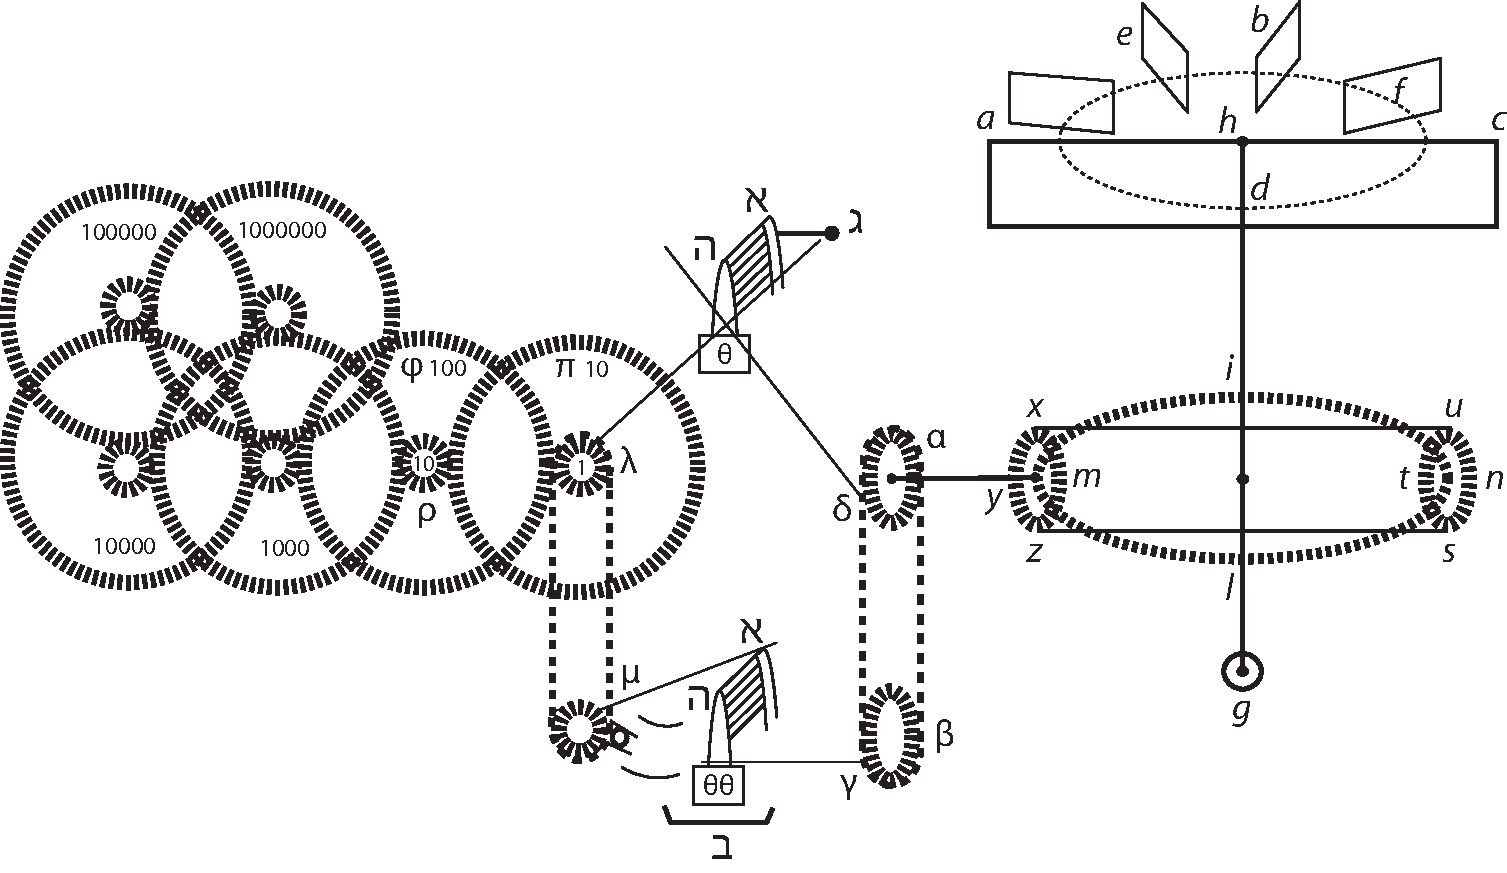
\includegraphics[width=1.0\textwidth]{images/LH037,05_092v-d1.pdf}\\
%\vspace{-4mm}
\begin{center}
  [\textit{Fig. 1}] 
  \end{center}\edtext{}{\lemma{\hspace{2mm}[\textit{Fig. 1}]}\killnumber\Cfootnote{Am unteren Ende der Kette $\displaystyle \alpha\beta\gamma\delta$ ist im Ms. ein zweites, hier nicht abgebildetes $\displaystyle \beta$ gezeichnet.}} 
  \pend
\pstart
\centering
Horologium \setline{1}Ventaneum\protect\index{Sachverzeichnis}{horologium ventaneum} perpetuum. 
\pend
\pstart
\noindent
Esto Rota\protect\index{Sachverzeichnis}{rota} Horizonti parallela $\displaystyle abcd$ semitecta et
\edtext{semiaperta, latus apertum $\displaystyle abc$. latus tectum}{\lemma{semiaperta,}\Bfootnote{\textit{(1)}\ pars tecta
\textit{(2)}\ latus
\textit{(a)}\ tectum
\textit{(b)}\ apertum [...] tectum
\textit{L}}}
\edtext{$\displaystyle adc$. Circumferentiae ejus
alae\protect\index{Sachverzeichnis}{ala}}{\lemma{$\displaystyle adc$.}\Bfootnote{\textit{(1)}\ alae in rota
\textit{(2)}\ Circumferentiae ejus alae
\textit{L}}}
infixae sunt
\edtext{$\displaystyle a$. $\displaystyle e$. $\displaystyle b$. $\displaystyle f$. $\displaystyle c$. etc.}{\lemma{}\Bfootnote{$\displaystyle a$. $\displaystyle e$. [...] etc.
\textit{ erg. L}}},
quae a vento\protect\index{Sachverzeichnis}{ventus} circumaguntur.
Ponatur enim $\displaystyle c$ esse oriens, $\displaystyle a$ occidens, $\displaystyle b$ septentrio, $\displaystyle d$ meridies.
Ventus orientalis $\displaystyle b$ aget versus $\displaystyle e$. occidentalis $\displaystyle b$ aget versus $\displaystyle f$. septentrionalis $\displaystyle a$ versus $\displaystyle d$. meridionalis $\displaystyle a$ versus $\displaystyle e$.
Eademque de caeteris ventis intermediis ratio est.
Ala\protect\index{Sachverzeichnis}{ala} autem $\displaystyle a$ eunte versus $\displaystyle e$. aut ala $\displaystyle f$ versus $\displaystyle b$.
alia ala ex latere tecto prodiens
\edtext{in ejus}{\lemma{in}\Bfootnote{\textit{(1)}\ earum
\textit{(2)}\ ejus
\textit{L}}}
locum succedit.
\pend
\pstart
Cur autem alterum latus tectum sit[,]
 ratio est ne ventus\protect\index{Sachverzeichnis}{ventus}
\edtext{in oppositas alas\protect\index{Sachverzeichnis}{ala} simul incidens}{\lemma{in}\Bfootnote{\textit{(1)}\ ejus alas incidens, vento
\textit{(2)}\ oppositas [...] incidens,
\textit{L}}},
sibi reluctetur.
Ut si ventus\protect\index{Sachverzeichnis}{ventus} septentrionalis a $\displaystyle b$ versus $\displaystyle d$ simul in alam\protect\index{Sachverzeichnis}{ala} $\displaystyle a$ et in oppositam $\displaystyle c$ incidat,
fiet aequilibrium, nec ratio erit cur huc potius quam illuc rota\protect\index{Sachverzeichnis}{rota} agatur[;]
\edtext{quemadmodum molendina aquatica\protect\index{Sachverzeichnis}{molendinum aquaticum} aquae immerguntur, nisi parte tantum, alioqui cursu ejus non circumagerentur, nisi debiliter, quod miror in
molendinis\protect\index{Sachverzeichnis}{molendinum} vulgaribus non observatum}{\lemma{}\Bfootnote{quemadmodum molendina aquatica\ \textbar\
\textit{(1)}\ in aquae libere po
\textit{(2)}\ in aquam
\textit{(3)}\ aquae\ \textbar\
immerguntur, [...] observatum
\textit{erg. L}}}.
\pend
\pstart
\edtext{Est ergo}{\lemma{Est ergo}\Bfootnote{\textit{erg. L}}}
Rota ventanea\protect\index{Sachverzeichnis}{rota ventanea} $\displaystyle abcd$ ita
\edtext{constructa ut quolibet vento\protect\index{Sachverzeichnis}{ventus} flante continue circumagatur}{\lemma{constructa}\Bfootnote{\textit{(1)}\ quolibet vento continue circumagetur
\textit{(2)}\ ut [...] circumagatur.
\textit{L}}}.
In quo differt ab Anemoscopio\protect\index{Sachverzeichnis}{anemoscopium},
aedibus imposito aut Gnomone ventaneo,\protect\index{Sachverzeichnis}{gnomon ventaneum}
quae a praesente vento moventur non nisi semel,
quando scilicet in lineam venti,\protect\index{Sachverzeichnis}{ventus} quo minus
\edtext{ei obstent, disponantur.}{\lemma{ei}\Bfootnote{\textit{(1)}\ obstet, disponatur
\textit{(2)}\ obstent, disponantur.
\textit{L}}}
\pend
\count\Bfootins=1000
\pstart
\begin{wrapfigure}[7]{l}{0.15\textwidth}
\vspace{-5mm}
     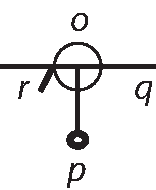
\includegraphics[trim = 0mm -3mm -5mm 0mm, clip, width=0.15\textwidth]{images/LH037,05_092v-d2.pdf}
     \centering
     [\textit{Fig. 2}] % \caption{Bildbeschreibung}
\end{wrapfigure}
Hujus Rotae ventaneae\protect\index{Sachverzeichnis}{rota ventanea} axis esto $\displaystyle gh$ mobilis cum rota $\displaystyle abcd$ in centro $\displaystyle g$ secumque movens rotam dentatam\protect\index{Sachverzeichnis}{rota dentata} $\displaystyle ilmn$ cui
\edtext{incumbit cylinder $\displaystyle mn$ desinens utrinque}{\lemma{incumbit}\Bfootnote{\textit{(1)}\ utrinque
\textit{(2)}\ cylinder [...] utrinque
\textit{L}}}
in tympana\protect\index{Sachverzeichnis}{tympanum}
\edtext{dentata $\displaystyle m$ et $\displaystyle n$ rotae\protect\index{Sachverzeichnis}{rota dentata}}{\lemma{dentata}\Bfootnote{\textit{(1)}\ $\displaystyle mn$
\textit{(2)}\ $\displaystyle m$ et $\displaystyle n$\
\textbar\ utrinque \textit{gestr.}\ \textbar\
rotae \textit{L}}}
extremitatibus incumbentia.
Horum tympanorum\protect\index{Sachverzeichnis}{tympanum} dentes\protect\index{Sachverzeichnis}{dens} ita comparati esse debent,
ut non nisi in unam partem cedant,
ubi autem cesserint et dentes rotae\protect\index{Sachverzeichnis}{rota dentata} praetermiserint,
se rursus erigant.
Exempli gratia dens\protect\index{Sachverzeichnis}{dens}
\edtext{$\displaystyle op$ circa centrum}{\lemma{$\displaystyle op$}\Bfootnote{%
\textit{(1)}\ infixus centr
\textit{(2)}\ circa centrum
\textit{L}}}
$\displaystyle o$ mobilis est solum versus $\displaystyle q$
non versus $\displaystyle r$ ob obstaculum $\displaystyle r$.
et si moveatur ab aliqua vi versus $\displaystyle q$.
ea discedente propria gravitate\protect\index{Sachverzeichnis}{gravitas} in $\displaystyle p$ appensa redit in situm priorem
%\begin{wrapfigure}[7]{l}{0.15\textwidth}
%\vspace{-5mm}
%     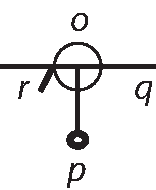
\includegraphics[trim = 0mm -3mm -5mm 0mm, clip, width=0.15\textwidth]{images/LH037,05_092v-d2.pdf}
%     \centering
%     [\textit{Fig. 2}] % \caption{Bildbeschreibung}
%\end{wrapfigure}
\edtext{perpendicularem. Ergo ponamus}{\lemma{perpendicularem.}\Bfootnote{%
\textit{(1)}\ Ergo unius Tympani,\protect\index{Sachverzeichnis}{tympanum} nempe $\displaystyle m$. dentes\protect\index{Sachverzeichnis}{dens} non sint mobiles nisi
\textit{(2)}\ Ergo ponamus
\textit{L}}}
ventum\protect\index{Sachverzeichnis}{ventus} [occidentalem]\edtext{}{\Bfootnote{occidenlatem \textit{\ L \"{a}ndert Hrsg.}}} agere rotam\protect\index{Sachverzeichnis}{rota alata}
\edtext{alatam}{\lemma{}\Bfootnote{alatam
\textit{erg. L}}}
hoc ordine $\displaystyle bcda$. aget dentatam\protect\index{Sachverzeichnis}{rota dentata} hoc ordine
\edtext{$\displaystyle inlm$. $\displaystyle i$ tendens}{\lemma{$\displaystyle inlm$.}\Bfootnote{%
\textit{(1)}\ Ergo
\textit{(2)}\ $\displaystyle i$ tendens
\textit{L}}}
per $\displaystyle n$ in $\displaystyle l$ non impediatur dentibus\protect\index{Sachverzeichnis}{dens} tympani\protect\index{Sachverzeichnis}{tympanum} horizontaliter incumbentis in $\displaystyle n$.
\edtext{quippe non cedentibus}{\lemma{quippe}\Bfootnote{%
\textit{(1)}\ mobilibus
\textit{(2)}\ non cedentibus
\textit{L}}}
ordine $\displaystyle nstu$
\edtext{seu sursum per latus meridionale quo nunc tendit rota dentata\protect\index{Sachverzeichnis}{rota dentata}, nisi cum toto cylindro sed serie $\displaystyle nuts$ seu sursum per latus septentrionale}{\lemma{}\Bfootnote{seu sursum
\textit{(1)}\ versus
\textit{(2)}\ per latus meridionale 
\textit{(a)}\ non vero serie $\displaystyle nuts $ seu sursum per latus septentrionale quo nunc impellit rota dentata\protect\index{Sachverzeichnis}{rota dentata} nisi cum toto cylindro
\textit{(b)}\ quo
\textit{(aa)}\ tendit
\textit{(bb)}\ nunc impellit rota dentata
\textit{(c)}\ quo nunc [...] septentrionale.
\textit{erg. L}}}.
At eodem motu $\displaystyle l$ tendens per $\displaystyle m$ in $\displaystyle i$ non impedietur dentibus\protect\index{Sachverzeichnis}{dens} tympani\protect\index{Sachverzeichnis}{tympanum} horizontaliter incumbentis in $\displaystyle m$.
\edtext{quippe itidem cedentibus sine toto cylindro}{\lemma{quippe}\Bfootnote{%
\textit{(1)}\ itidem mobilibus tantum serie
\textit{(2)}\ itidem 
\textit{(a)}\ serie non mobilibus
\textit{(b)}\ cedentibus [...] cylindro
\textit{L}}}
sursum per latus septentrionale seu serie
\edtext{$\displaystyle mxyz$ quo nunc tendit rota dentata,\protect\index{Sachverzeichnis}{rota dentata}\textso{ sine toto cylindro }non vero sursum}{\lemma{$\displaystyle mxyz$}\Bfootnote{%
\textit{(1)}\ quo parte nunc tendit rota, \textso{nisi cum toto cylindro}
\textit{(2)}\ quo nunc [...] \textso{cylindro}
\textit{(a)}\ sed tantum deorsum
\textit{(b)}\ non vero sursum
\textit{L}}}
per latus meridionale seu serie $\displaystyle mzyx$
\edtext{nisi cum toto cylindro}{\lemma{}\Bfootnote{%
nisi [...] cylindro
\textit{ erg. L}}}.
Ergo Cylinder circumagetur sursum in
\edtext{latus meridionale}{\lemma{latus}\Bfootnote{%
\textit{(1)}\ septentrionale
\textit{(2)}\ meridionale
\textit{L}}}
serie $\displaystyle nstu$ seu $\displaystyle mzyx$. Contra ponatur vento\protect\index{Sachverzeichnis}{ventus} verso Rota alata\protect\index{Sachverzeichnis}{rota alata} verti
[93~r\textsuperscript{o}]
ordine $\displaystyle badc$ et rota dentata\protect\index{Sachverzeichnis}{rota dentata}
\edtext{serie $\displaystyle imln$.}{\lemma{serie}\Bfootnote{%
\textit{(1)}\ $\displaystyle lnim$.
\textit{(2)}\ $\displaystyle imln$.
\textit{L}}}
\edtext{$\displaystyle i$ tendens}{\lemma{$\displaystyle i$}\Bfootnote{%
\textit{(1)}\ veniens
\textit{(2)}\ tendens
\textit{L}}}
per $\displaystyle m$ versus $\displaystyle l$ dentibus\protect\index{Sachverzeichnis}{dens} Tympani\protect\index{Sachverzeichnis}{tympanum} in $\displaystyle m$. quippe
versus \edtext{$\displaystyle z$. non cedentibus nisi cum cylindro tenebitur;
at $\displaystyle l$ tendens per $\displaystyle n$ in $\displaystyle i$ non tenebitur dentibus\protect\index{Sachverzeichnis}{dens} tympani\protect\index{Sachverzeichnis}{tympanum} in $\displaystyle n$. quippe cedentibus versus $\displaystyle u$ sine toto cylindro, cylinder ergo}{\lemma{$\displaystyle z$.}\Bfootnote{%
\textit{(1)}\ mobilibus
\textit{(2)}\ cedentibus non tenebitur; at $\displaystyle l$ tendens per $\displaystyle n$ in $\displaystyle i$ tenebitur 
\textit{(a)}\ tympanis 
\textit{(b)}\ dentibus tympani in $\displaystyle n$. quippe non cedentibus versus $\displaystyle u$. 
\textit{(aa)}\ Impelle 
\textit{(bb)}\ Ergo cylinder 
\textit{(cc)}\ nisi cum toto cylindro, cylinder ergo
\textit{(3)}\ non cedentibus [...] versus $\displaystyle u$ 
\textit{(a)}\ et s 
\textit{(b)}\ sine [...] ergo 
\textit{L}}}
agetur ab $\displaystyle n$ versus $\displaystyle s$
seu \edtext{ordine $\displaystyle nstu$}{\lemma{ordine}\Bfootnote{%
\textit{(1)}\ $\displaystyle nuts$
\textit{(2)}\ $\displaystyle nstu$
\textit{L}}}
quo prius agebatur. Utcunque
ergo moveatur Rota alata\protect\index{Sachverzeichnis}{rota alata} $\displaystyle abcd$. cylinder semper
agetur \edtext{serie $\displaystyle nstu$}{\lemma{serie}\Bfootnote{%
\textit{(1)}\ $\displaystyle nuts$
\textit{(2)}\ $\displaystyle nstu$
\textit{L}}}
\edtext{seu [$mzyx$]}{\lemma{seu}\Bfootnote{%
\textit{(1)}\ $\displaystyle txyz$
\textit{(2)}\ $mzyz$ 
\textit{L \"{a}ndert Hrsg.}}}
ac proinde catena\protect\index{Sachverzeichnis}{catena}
qua ventus\protect\index{Sachverzeichnis}{ventus} pondus\protect\index{Sachverzeichnis}{pondus}
relevat semper movebitur serie
\edtext{$\displaystyle \alpha\beta\gamma\delta$.\\
\hspace*{7,5mm}
Efficiamus}{\lemma{$\displaystyle \alpha\beta\gamma\delta$.}\Bfootnote{%
\textit{(1)}\ Supponatur
\textit{(2)}\ Efficiamus
\textit{ L}}}
nunc \edtext{pondus\protect\index{Sachverzeichnis}{pondus} $\displaystyle \theta$ vix integro mense pervenire ex $\displaystyle \theta$ in $\displaystyle \theta\theta$}{\lemma{pondus $\displaystyle \theta$}\Bfootnote{%
\textit{(1)}\ descendisse
\textit{(2)}\ integrum mensem absolvere debere antequam perveniat ex $\displaystyle \lambda$ in $\displaystyle \mu$
\textit{(3)}\ vix [...] in $\displaystyle \theta\theta$.
\textit{L}}}.
Id ita fiet
\edtext{si catena\protect\index{Sachverzeichnis}{catena}}{\lemma{si}\Bfootnote{%
\textit{(1)}\ rota\protect\index{Sachverzeichnis}{rota}
\textit{(2)}\ catena
\textit{L}}}
in qua descendit $\displaystyle \lambda\mu$. tympanum\protect\index{Sachverzeichnis}{tympanum} $\displaystyle \lambda$ cui circumposita est circumagere
debeat, et tympanum $\displaystyle \lambda$ rotam $\displaystyle \pi$ decuplo se majorem,
concentricam, ergo decies citius. Rota\protect\index{Sachverzeichnis}{rota} $\displaystyle \pi$ circumaget sive catena\protect\index{Sachverzeichnis}{catena}
sive dentibus\protect\index{Sachverzeichnis}{dens} sibi junctam rotulam decies se minorem, $\displaystyle \rho$. et quia
eccentricam ideo aequivelociter, ergo motus Rotulae $\displaystyle \rho$ erit ut
10. convertetur enim decies, dum $\displaystyle \pi$ semel, quia et decuplo minor.
At rotula $\displaystyle \rho$ decies
\edtext{conversa[,] Rota\protect\index{Sachverzeichnis}{rota}}{\lemma{conversa[,]}\Bfootnote{%
\textit{(1)}\ rotula
\textit{(2)}\ Rota
\textit{L}}}
\edtext{ejus concentrica $\displaystyle \phi$ decuplo major}{\lemma{ejus}\Bfootnote{%
\textit{(1)}\ decuplo major concentrica
\textit{(2)}\ concentrica [...] major
\textit{L}}}
itidem decies convertetur, quia ei affixa.
Ergo dum $\displaystyle \pi$ convertitur semel $\displaystyle \phi$ ei aequalis convertetur
decies. Erit ergo motus ejus decuplo major quam $\displaystyle \pi$ qui est
ut 10. seu erit ut 100. Ergo tertia habebit
celeritatem\protect\index{Sachverzeichnis}{celeritas}
ut 1000, et quarta ut 10,000, et quinta ut 100,000
et sexta ut 1000,000. Sed si eo usque
\edtext{procedere consultum}{\lemma{procedere}\Bfootnote{%
\textit{(1)}\ opus
\textit{(2)}\ consultum
\textit{L}}}
futurum non sit.
Ex his patet pondus\protect\index{Sachverzeichnis}{pondus} $\displaystyle \theta$ si
per solam catenam\protect\index{Sachverzeichnis}{catena} $\displaystyle \lambda\mu$ in tympano\protect\index{Sachverzeichnis}{tympanum} $\displaystyle \lambda$ positam
\edtext{cum circulo $\displaystyle \pi$ circumagens}{\lemma{cum [...] circumagens}\Bfootnote{\textit{erg. L}}}
descensurum sit minuto
\edtext{uno, circulo}{\lemma{uno}\Bfootnote{%
\textit{(1)}\ . Ea multiplicatione rotarum\protect\index{Sachverzeichnis}{rota} cont
\textit{(2)}\ , circulo
\textit{L}}}
quoque $\displaystyle \phi$ circumacto vix descensurum minutis 10. et
circulo 1000 minutis 100. et circulo 10,000 minutis 1000, et 
circulo 100,000 minutis 10,000, et circulo 1000,000 minutis 
100,000. id est plus quam
\edtext{mensibus duobus}{\lemma{mensibus}\Bfootnote{%
\textit{(1)}\ tribus
\textit{(2)}\ duobus.
\textit{L}}}.
Est enim mensis minutorum 43,200.
Sed septimana sufficit seu minuta 10,000. 
Nunquam enim septimana
\edtext{erit in qua ventus\protect\index{Sachverzeichnis}{ventus} non ponderi\protect\index{Sachverzeichnis}{pondus} ex $\displaystyle \theta\theta$ in $\displaystyle \theta$ elevando sufficiat}{\lemma{erit}\Bfootnote{%
\textit{(1)}\ sine vento qui postea
\textit{(2)}\ in qua [...] sufficiat.
\textit{L}}}.
Ausim dicere nec
diem fore[,] ita suffecerint mille minuta seu 4 rotae.\protect\index{Sachverzeichnis}{rota}
Sed necesse est pondus\protect\index{Sachverzeichnis}{pondus} amplius ponderare, quam rota 10,000 decies
millies, et quam rota 1000 millies, et quam rota $\displaystyle \phi$ centies, et
quam rota $\displaystyle \pi$ decies, seu 11,111 libras, si rota quaelibet ponatur
esse per se unius librae. Sed si quaelibet rota\protect\index{Sachverzeichnis}{rota} sit decem librarum
ponderabit \edtext{111,110 \Pfund. Quod nimium. Adhibendae}{\lemma{111,110 \Pfund.}\Bfootnote{%
\textit{(1)}\ Sunt
\textit{(2)}\ Quod nimium. Adhibendae
\textit{L}}}
ergo aliae tardandi rationes. Esto
\edtext{Horologium\protect\index{Sachverzeichnis}{horologium} ordinarium diurnum[,]
augeatur illi spatium descensus}{\lemma{Horologium}\Bfootnote{%
\textit{(1)}\ quod currit m
\textit{(2)}\ ordinarium diurnum[,]
\textit{(a)}\ detur illi spatium descensus
\textit{(b)}\ augeatur [...] descensus
\textit{L}}}
quantum commode licet, sit v.g. 100 pedum.
Horologium\protect\index{Sachverzeichnis}{horologium} quod decem
\edtext{diebus decurrat}{\lemma{diebus}\Bfootnote{%
\textit{(1)}\ currat
\textit{(2)}\ decurrat,
\textit{L}}},
\edtext{circumvolvatur rectum 100 pedum}{\lemma{circumvolvatur}\Bfootnote{%
\textit{(1)}\ lineae decem
\textit{(2)}\ rectum 100 pedum
\textit{L}}}
spiralis 1000 pedum. Manifestum est pondus\protect\index{Sachverzeichnis}{pondus} in ea
decuplo longius moraturum. Habebimus ergo 100 dierum
horologium\protect\index{Sachverzeichnis}{horologium}.
Erit \edtext{fateor et}{\lemma{fateor et}\Bfootnote{\textit{erg. L}}}
virium decuplo minorum, sed sufficit
ei satis virium esse ad indicem quendam circumagendum,
aut Elaterium\protect\index{Sachverzeichnis}{elaterium}
quoddam soni edendi causa aperiendum etc.
\pend
\count\Bfootins=1200
\pstart
Sed quid huc imus, certum est non esse diem, in quo
non sit ventus\protect\index{Sachverzeichnis}{ventus} unius horae. At debilis, sed illum fortem
reddemus capiendo velut in Tubum, alisque\protect\index{Sachverzeichnis}{ala} grandioribus
factis. Denique sufficit Horologium esse, septimanae,
aut decendii: sumto Horologio ordinario\protect\index{Sachverzeichnis}{horologium} unius diei, ac
decuplicato.
\pend
\vspace{2em}
\pstart
\noindent
\textit{Auf der oberen rechten Spalte von Bl. 93~r\textsuperscript{o}:}
\pend
\vspace{0.5em}
\pstart
\noindent
Quoad elevationem et depressionem. U$\displaystyle\langle$tique$\displaystyle\rangle$
ut pondus\protect\index{Sachverzeichnis}{pondus} in $\displaystyle \theta\theta$.
\edtext{stylus $\displaystyle \mu$\hebr{'}
 impingens in}{\lemma{stylus}\Bfootnote{%
\textit{(1)}\ in
\textit{(2)}\ $\displaystyle \mu$\hebr{'}
  impingens in
\textit{L}}}
tympa$\displaystyle\langle$num $\displaystyle \mu \rangle$
elaterio\protect\index{Sachverzeichnis}{elaterium} descendens deponet pondus quod $\displaystyle\langle$---$\displaystyle\rangle$
\hebr{'}
  tenebat in repositorium \hebr{b}
   atque ita abibit.
Eodem momento pondus aliud ei aequale et simile
positum in unco \hebr{g}
 ansa eadem, ab eo liberatum
ob communicationem Elaterii unci cum Elaterio\protect\index{Sachverzeichnis}{elaterium}
styli $\displaystyle \mu$\hebr{'} 
et ita incidet pondus $\displaystyle \theta$ in stylum $\displaystyle \lambda\theta$
continuabitque circumagere rotam.\protect\index{Sachverzeichnis}{rota} Interea pondus
$\displaystyle \theta\theta$ in repositorio \hebr{b}
 expectabit dum stylus $\displaystyle \gamma\theta\theta$ 
veniens a $\displaystyle \beta$ versus $\displaystyle \delta$
\edtext{cylindro a vento\protect\index{Sachverzeichnis}{ventus} circumacto}{\lemma{cylindro [...] circumacto}\Bfootnote{\textit{erg. L}}}
pondus\protect\index{Sachverzeichnis}{pondus} $\displaystyle \theta\theta$ ansa \hebr{h} apprehensum
attollat in $\displaystyle \delta\theta$. ubi stylus $\displaystyle \delta\theta$ Elaterium\protect\index{Sachverzeichnis}{elaterium}
suum impulsum in tympanum\protect\index{Sachverzeichnis}{tympanum} $\displaystyle \alpha$ laxans remittensque
seu \edtext{delabens pondus}{\lemma{delabens}\Bfootnote{%
\textit{(1)}\ rotam
\textit{(2)}\ pondus
\textit{L}}}
ansa n. %\edtext{}{\lemma{n.}\Cfootnote{enim}} % PR: Diese Fußnote bitte ignorieren!
relinquat in unco \hebr{g}
 quem praetervecta erat ansa,
quia uncus \hebr{g}
 semper sursum mobilis est, non
nisi Elaterio\protect\index{Sachverzeichnis}{elaterium} liberato deorsum. Non est opus Elaterio\protect\index{Sachverzeichnis}{elaterium} styli $\displaystyle \mu$\hebr{'} 
\edtext{quia stylus}{\lemma{quia}\Bfootnote{%
\textit{(1)}\ ipsummet $\displaystyle \eta$
\textit{(2)}\ stylus
\textit{L}}}
deposito pondere\protect\index{Sachverzeichnis}{pondus} in repositorio ob ansam infra apertam[,]
deprimens a. %\edtext{}{\lemma{a.}\Cfootnote{autem}} % PR: Diese Fußnote bitte ignorieren!
repositorium aperiet uncum.
\pend
\vspace{2em}
\pstart
\noindent
\textit{Am oberen Rand von Bl. 92~v\textsuperscript{o}, über} [\textit{Fig. 1}]:
\pend
\vspace*{0.5em}
\pstart
\noindent
Nunc nimium nunc parum venti\protect\index{Sachverzeichnis}{ventus} habemus.
Ergo interest $\displaystyle\langle$saepe motum$\displaystyle\rangle$ superfluum velut in aerarium publicum referri.
Sed quomodo motum[,] rem transitoriam?
Si dicam?
Si efficiamus ut moveat aliquid,
quod postea se restituens,
ubi volemus,
motum nobis repraesentet.
Motum a. %\edtext{}{\lemma{a.}\Cfootnote{autem}} % PR: Diese Fußnote bitte ignorieren!
in aerarium referre possumus,
si gravia\protect\index{Sachverzeichnis}{grave} levari,
Elastica\protect\index{Sachverzeichnis}{elasticum} comprimi aut tendi faciamus. Gravia levanda vel multa vel alte.
Nam si non alte aut pauca, subito se restituent.
Si tarde debiliter movebunt, perdita vi per attrectationes, utique inutiliter.
\pend
\pstart
Omnis ars hominum in eo consistit ut eorum quae natura nobis dedit,
nihil otiosum esse sinamus.
Hinc etiam etsi per machinas\protect\index{Sachverzeichnis}{machina}
nihil lucramur,
\edtext{sed temporis}{\lemma{sed}\Bfootnote{%
\textit{(1)}\ tempus
\textit{(2)}\ temporis
\textit{L}}}
tantum perdamus, quantum loci lucramur,
in eo tamen lucratos nos putamus, quod non perdidimus,
nam tempus hoc alioquin nobis periisset, aut in alia tamen utilia fuisset absumtum.
Similiter in machinis\protect\index{Sachverzeichnis}{machina} contrariis ubi multa simul aguntur,
v.g. ubi homo tantum agit quantum 10. nihil lucramur,
nam vires majores impendimus,
sed quia vires eae alioquin fuissent otiosae lucrum reputamus.
\pend
\vspace*{2em}
\pstart
\noindent
\textit{Nebenrechnungen am Rand:}
\pend
\vspace*{0.5em}
\pstart
\noindent
\begin{minipage}[t]{0.3\textwidth}
\vspace{-2.5mm}
$\begin{array}{ll}
& \, \, \, \, 24\\
& \, \, \, \, \, \, \, 30\end{array}\\
\begin{array}{ll}
\hline 
& \, \, \, \, 7200\\
& \, \, \, \, \, \, \, 6\end{array}\\
\begin{array}{ll}
\hline 
& 43200\end{array}$
\end{minipage}
\begin{minipage}[t]{0.3\textwidth}
\noindent
100\\
$\begin{array}{ll}
&\, \, \, \, \, \, \, \, 365
\\
&\, \, \,  \, \, \, \, \, \, \, \, 720\end{array}
\\
\begin{array}{ll}
\hline 
& \, \, \, \, \, \, \, 7300
\\
& 2255\end{array}
\\
\begin{array}{ll}
\hline 
& 262800
\\
& \, \, \, \, \, \, \, \, \, \, 2\end{array}\\
\begin{array}{ll}
\hline 
& 525600\end{array}$
\end{minipage}
\pend
\count\Bfootins=1500